\documentclass[twocolumn]{article}
\usepackage{times}
\usepackage{graphicx}

\begin{document}

\title{Garage MEMS: DIY fabrication of a 10um pitch comb drive}
\author{Andrew Zonenberg\\
	Rensselaer Polytechnic Institute\\
	110 8th Street\\
	Troy, New York U.S.A. 12180\\
	\texttt{zonena@cs.rpi.edu}}
\date{\today}
\maketitle

\begin{abstract}
\paragraph*{}
To be written...
\end{abstract}

\section{Introduction and related work}
\paragraph*{}
The goal of this work was to design and fabricate a MEMS comb drive at 10$\mu m$ pitch, from a
single piece of silicon (without wafer bonding or similar processes) using equipment and supplies
available to a dedicated hobbyist. By doing this, the author hopes to remove the stigma of
difficulty traditionally associated with microfabrication and increase interest in the subject
among amateurs.

\paragraph*{}
\cite{OfficePrint} describes a method for using a 600dpi laser printer and photographic reduction to
create photomasks for large-feature-size lithography. This method still requires the use of a
contact aligner in a cleanroom for exposure, however. The author improved on this method in
\cite{DiyFab} by printing on overhead transparency film and performing the reduction with a
modified metallurgical microscope to get slightly smaller feature sizes. Since writing that paper
the author has been improving the $5 \mu m$ process to increase yields.

\section{Process outline}

\subsection{Bulk etching and hardmask}
\paragraph*{}
One of the problems facing a hobbyist microfabrication lab is the lack of RIE capability, requiring
wet etching for all patterning. $KOH$-IPA-water has been widely characterized in the literature (for
example \cite{SmoothWalls}) as an anisotropic etch that is very selective for $<100>$ and $<110>$
planes and has a much lower etch rate along the $<111>$ plane.

\paragraph*{}
Many common positive photoresists, such as the Shipley SP24 used in this paper, use weak alkaline
solutions as a developer (the author typically uses a 1\% wt. solution of $NaOH$ in distilled water)
and will not survive exposure to the far more concentrated (25\% $KOH$) alkalis used for etching of
$Si$. Thermal oxide can be used as a hardmask for shallow etches, but $SiO_2$ is slowly etched by
$KOH$ and is not suitable for deep ($>10 \mu m$) etches; typical processes for deep etching use
$Si_3N_4$ deposited by low-pressure chemical vapor deposition (LPCVD) as a hardmask.

\paragraph*{}
Due to the lack of LPCVD capabilities the author was forced to select an alternate hardmask.
Preliminary research suggested that $Ta_2O_5$ might be a suitable choice as it has been reported by
\cite{Christiansen} and others to be extremely resistant to $KOH$ but can be etched by dilute $HF$
solutions. \cite{Nanodots} also demonstrated the use of $Ta_2O_5$ as a hardmask for reactive ion
etching (RIE). Furthermore, $Ta_2O_5$ can be deposited by the sol-gel method (\cite{Dielectric}).
The author selected Emulsitone Tantalumfilm for this experiment, which does not specifically mention
$KOH$ in the datasheet (\cite{Taf}) but will dissolve in 10\% $HF$ in 100 sec.

\paragraph*{}
Since $<110>$ Si does not cleave along perpendicular axes (the $<111>$ planes are at 70.5 and 109.5

\subsection{Wafer thinning}
\paragraph*{}
The maximum aspect ratio achieved by \cite{SmoothWalls} was approximately 10. At $5 \mu m$ feature
size, this limits the maximum height of the comb drive fingers to around $50 \mu m$. This is too
thin to be easily handled so a support structure will be added around the rim of the device.

\paragraph*{}
Both sides of the wafer are masked with $Ta_2O_5$ and photoresist, then the back side is patterned
by projection lithography with a mask containing a square cutout surrounded by a ~1mm square ring.
After developing and hardmask etching the wafer is etched from back to front until the central
portion of the die has been thinned to around $80 \mu m$ (Fig. ~\ref{xc1}). After a second
photoresist coating, the front side of the die is patterned with the comb drive pattern and the
hardmask is etched; leaving the thinned portion of the wafer unprotected. The die is then etched
from both sides until punctured, leaving the comb drive fingers on a $40 \mu m$ membrane
(Fig. ~\ref{xc2}) surrounded by a 1mm ring of $525 \mu m$ Si for handling.

\begin{figure}[h!]
\begin{center}
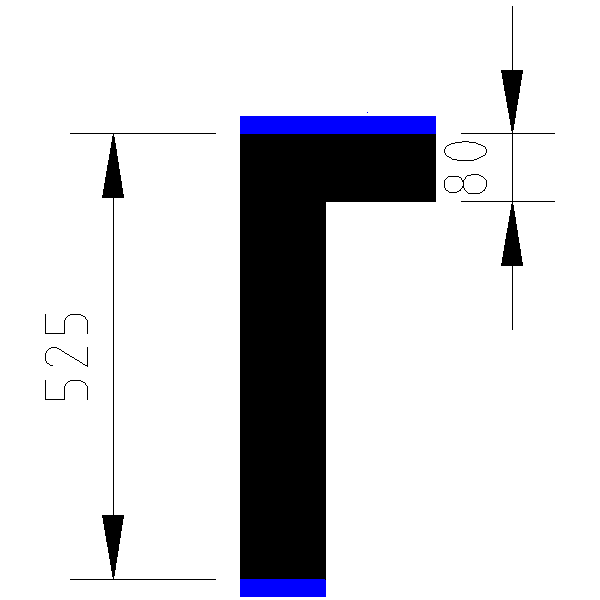
\includegraphics[scale=0.25]{CrossSection1.png}
\end{center}
\caption{Cross section after backside etch. $Si$ is shown in black, hardmask blue. Hardmask
thickness exaggerated for clarity.}
\label{xc1}
\end{figure}

\begin{figure}[h!]
\begin{center}
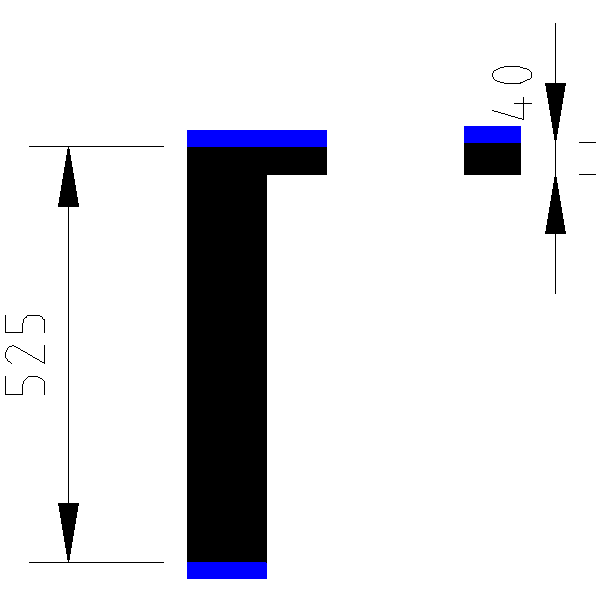
\includegraphics[scale=0.25]{CrossSection2.png}
\end{center}
\caption{Cross section after through-wafer etch.}
\label{xc2}
\end{figure}

\subsection{Metalization}
\paragraph*{}
Depositition paragraph to be written...

\paragraph*{}
After metalization the wafer is spin coated in photoresist (being sure to apply a suitable excess
of resist to coat sidewalls of the fingers) and patterned by projection lithography followed by
etching in a $HCl:H_2O_2:H_2O$ solution to separate the contact areas.


\section{Experimental setup and results}
\paragraph*{}
To be written...

\section{Conclusions}
\paragraph*{}
To be written...

\section{Future work}
\paragraph*{}
To be written...

\section{Acknowledgements}
\paragraph*{}
To be written...

\begin{thebibliography}{99}
	\bibitem{OfficePrint}
	Tao Deng, Hongkai Wu, Scott T. Brittain, George M. Whitesides, ``Prototyping of Masks, Masters,
	and Stamps/Molds for Soft Lithography Using an Office Printer and Photographic Reduction",
	Anal. Chem. 2000, 72, 3176-3180
	
	\bibitem{DiyFab}
	Andrew Zonenberg, ``DIY fabrication of microstructures by projection photolithography",
	self-published, 2011. Available: http://colossus.cs.rpi.edu/~azonenberg/papers/litho1.pdf
	
	\bibitem{SmoothWalls}
	V. K. Dwivedi, R. Gopal, S. Ahmad, ``Fabrication of very smooth walls and bottoms of silicon
	microchannels for heat dissipation of semiconductor devices", Microelectronics Journal
	Volume 31, Issue 6, 30 June 2000, Pages 405-410 
	
	\bibitem{Christiansen}
	Christiansen et al, ``Tantalum oxide thin films as protective coatings for sensors", MEMS '99
	
	\bibitem{Nanodots}
	Ik Hyun Park, Jang Woo Lee, Chee Won Chuang, ``Formation of Silicon Nanodot Arrays by Reactive
	Ion Etching Using Self-Assembled Tantalum Oxide Mask", 2005, J. Ind. Eng. Chem., Vol. 11, No. 4,
	590-593
	
	\bibitem{Dielectric}
	C. Chaneliere, J. L. Autran, R. A. B. Devine, B. Balland, ``Tantalum pentoxide ($Ta_2O_5$) thin
	films for advanced dielectric applications", 1998, Materials Science and Engineering, R22,
	269-322
	
	\bibitem{Taf}
	Emulsitone, ``Emulsitone Tantalumfilm", accessed Jun 2 2011. Available:
	http://emulsitone.com/taf.html
	
\end{thebibliography}

\end{document}
